\documentclass[article]{aaltoseries}
\renewcommand{\thesection}{\Roman{section}} 
\usepackage[utf8]{inputenc}
\usepackage{algpseudocode}
\usepackage{amssymb}
\usepackage{amsmath}
\usepackage{algorithm}
\makeatletter
\newcommand*{\rom}[1]{\expandafter\@slowromancap\romannumeral #1@}
\makeatother

\begin{document}
%=========================================================

\title{Using reinforcement learning to learn gaming strategies}
\author{Group Name: Cautious Train\\\\Dongmin Wu, 605308, dongmin.wu@aalto.fi% Your first and last name: do _not_ add your student number
\\{Shan Kuan, 604888, shan.kuan@aalto.fi}} % Your Aalto e-mail address

\maketitle
%==========================================================
\begin{abstract}
Artificial Intelligence is the technology that makes the machine to work in intelligence way and then to aid our daily life more easily. However, in the research of the Artificial Intelligence industry, the amount of data and the quality of the data, which are domains the accuracy of the result in the machine learning industry. In this project, we introduce the Reinforcement learning, which is the way that researcher does not need to collect the training data before the training step. In other words, the machine learns the rule of conduct without the supervisor, and then to generate the training data during the training step.

In this study, we analyzed two leading methods from the reinforcement learning, which are Deep Q-learning and Policy Gradients, to introduce the core ideal of each method. In deep q-learning, it is a value-based method. It tries to maximal the expected future rewards via learning of a state-action q function. On the other side, policy gradients are policy-based methods. The goal of this method is to find the optimal policy by directly optimizing of the policy function.

In the experimental, this project conducts the simple grid game to elaborate the algorithms. Therefore, the study will discuss the weakness and strength between deep q-learning and policy gradients in different application circumstance. 
  
\end{abstract}


%============================================================


\section{Introduction}

In this project, we specifically introduce two well known methods in the reinforcement learning, which is q-learning and policy gradient. Q-learning is the traditional reinforcement learning algorithm, it uses the reward function to evaluate the action and then to obtain the state in the next. For the reward function, it is not the function to tell the machine how to act. In contrast, it tells the machine what outcomes are desired or undesired in the current circumstance. In 1989, a computer scientist named Chris Watkins \cite{Watkins1992}, he introduces the innovation ideal to combine the Bellman equation and the law of fact to generate the new type of learning algorithm, which is Q-learning.

In the big family of reinforcement learning, most of the methods do not have convergence guarantees after numerous of regression procedure. If the testing environment is trivial, the q function would convergence in a short term of regression. However, if the testing environment is complexity, it has plenty of different state and action that would cause the time to find the optimal policy. According to the policy gradient \cite{Sutton:1999:PGM:3009657.3009806}, the method does not suffer convergence problem. It uses a neural network to approximate the Q function and then directly optimizes in the policy space. During the repeat process, in the end, the policy gradient would converge to the optimal policy.

Throughout this work, we will implement the two most popular methods of reinforcement learning algorithms, deep q-learning, and policy gradient, in learning to play the maze game. During the training step, the game agent can learn how to escape the ghost and the obstacle and then to reach the final destination. In section \rom{3}, the report introduces the methods deep q-learning and policy gradient \cite{mnih2015humanlevel} to approximating the Q function through different based on reinforcement learning. In section \rom{4}, we will introduce the training environment, the maze game, what is the reward and penalty in the game. Therefore, how to train an agent reach the goal in the training stage. In section \rom{5}, to discuss the correlation of the hyper-parameter of deep q-learning and policy gradient. In section \rom{6}, the evaluation provides further discussion between deep q-learning and policy gradient. In section \rom{7}, the report analyzes trivial and complex environment with two methods. Furthermore, regarding the test result to discuss the weakness and strength of two methods.



%============================================================


\section{Related Work}

Reinforcement learning (RL) is a big family, according to the different circumstance; reinforcement learning provides the different method to address the specific problem. Except the well known method, q-learning and policy gradient, the following research will introduce the other method on several different schemes.

In 1995, Gerald Tesauro \cite{Tesauro:1995:TDL:203330.203343} proposed a new RL methods, TD-Gammon, it is a well known method to play backgammon game. As same as the q-learning, TD-gammon used the model-free RL to approximated the value function. Therefore, TD-gammon also include the method of using a multilayer perceptron with one hidden layer to advance the performance of calculate the value function. However, TD-gammon only work well in the backgammon game, but failed in the other board game, such as Go and checkers. According to the research \cite{Tesauro1992}, TD-gammon is not able to converge as it may get stuck in the locally optimal solution.
 
SARSA stands for State-Action-Reward-State-Action. In 1994, SARSA developed by Rummery and Niranjan \cite{articleonline}, which is the on-line policy learning of RL. Therefore, SARSA takes into account of the prediction state from the control policy during the learning step. In contrast, q-learning is the off-line policy, and it does not guarantee to follow the optimal state that predict by the control policy. To compare the result of two methods, although SARSA needs to keep the action value longer in the stored before the new updated. It provides the way to escape the local optimal and received the higher reward in the end of the regression.



%------------------------------------------------------------


\section{Method}


The method we used in this reinforcement learning project is basically comparison. We will designed an environment of the game and run different algorithm on it. The evaluation of algorithms will be based on the curve of how many reward score in average the algorithm can earn. In this section, we will explain the environment we used and elaborately describe the implement of our algorithms. 


The first algorithm we use in this project is Deep Q Learning, where the agent will learn a good solution through evaluating and updating the quality of each state. 

\begin{equation} \label{eq:q_learning}
  Q(s,a) = r + \gamma (max(Q(s\prime ,a\prime ))
\end{equation}



$Q$ is the quality of current state, and $Q\prime$ is the quality of all the possible state that can be reached from current state. This is the Bellman Equation, which shows the relationship between the quality of current state and quality of all  possible next state.

Since we already have the approach of how to get quality of one state from its future states, we can build a neural network to predict quality Q of future states and compare this with the actual quality Q-target which derived from Bellman Equation



\begin{equation} \label{eq:q_loss}
  Loss = \Sigma (Q_{target}(s,a)) - Q \prime (s,a))^2
\end{equation}



For better prediction, we used the Dueling DQN algorithm. 
As the Algorithm \ref{alg:q-learning} shows, this approach has two neural network, the primary network will predict the quality of next states of s’ and choose an action from it. The target network is used to predict the quality value Q’. The primary controls the direction of agent and the target network calculates the rewards in that direction




\begin{algorithm}
  \caption{Dueling DQN}
  \label{alg:q-learning}
  \begin{algorithmic}[1]
    \Repeat
      
      \State $Q \gets PrimaryNetwork(s)$  

      \State $s\prime \gets Environment(max(Q(s)))$

      \State $Q_{direction} \prime \gets PrimaryNetwork(s \prime)$ 

      \State $Q_{value} ,r \prime \gets TargetNetwork(s \prime)$
      
      \State $Q_{target} = r + \gamma Q_{value}[max(Q_{direction})]$

      \State $\theta_{Primary} \gets \theta_{Primary}  + \nabla \alpha \Sigma (Q_{target}(s,a)) - Q \prime (s,a))^2$ 

    \Until Exceed the maximal episode
  \end{algorithmic}
\end{algorithm}



 

The policy gradient we used is a base on the equation below:

\begin{equation} \label{eq:q_loss}
  Loss = -log(\pi) \times A
\end{equation}

In the equation, the $\pi$ presents the policy we will choose in a state, 
or more intuitively, it means the chance of the agent choosing certain action 
based on its current state.

The parameter $A$ represents the advantage of the policy, 
which is an combination with the rewards got from the game 
and the baseline of our expectation. The base could be changed in different scenario.

Algorithm \ref{alg:policy} shows the pseudocode of policy gradient. 



\begin{algorithm}
  \caption{Policy Gradients}
  \label{alg:policy}
  \begin{algorithmic}[1]
    \Repeat

      \For {step = 1 to MAX STEPS}
      
      \State $a \gets PolicyNetwork(s)$  

      \State $s\prime ,r \gets Environment(a)$

      \State $Buffer.append(s, a, s\prime, r)$ 

      \If {terminated}
        \State $v \gets r_0+ \gamma r_1 + \gamma^2 r_2 ... \gamma^i r_i (\gamma < 1, i \in [0,Buffer.size()-1]) $
        \State $\theta_{Primary} \gets \theta_{Primary} + \nabla \alpha log(\pi) \times v$
      \EndIf
      \EndFor

    \Until Exceed the maximal episode
  \end{algorithmic}
\end{algorithm}


%------------------------------------------------------------


\section{Data}

Since the goal of our project is comparing the two currently popular Reinforcement 
Learning algorithms, we decided to make a tiny game that we can test these two algorithms.
 The game we created is simple which is based on a grid map. 
 In the map there are 3 points: Trophy, Pitfall and Hero, only the play is controllable. 
 The goal for this game is directing the Hero reach the Trophy, avoiding the Pitfall 
 in the the map. 
 
 Figure \ref{fig:map} shows an example of of the map. In addition, the policy of the environment could be changed for different experiment.

\begin{figure}[t!]
  \begin{center}
    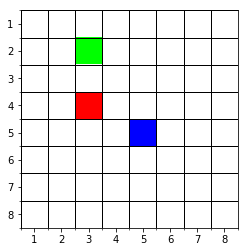
\includegraphics[width=0.3\textwidth]{figures/grid_drew}
    \caption{Example of the game we used in this project}
    \label{fig:map}
  \end{center}
\end{figure}

%------------------------------------------------------------


\section{Experiments}

We first designed the task we want the algorithm and the learning goal based on these task: 
\begin{itemize}
\item \textbf{Normal Task}
Description: In each episode the map is fixed; position of pitfall is fixed; the size of map is normal (8*8).
Learning Goal:  Algorithm will find a path to the goal properly

\item \textbf{Extremely Task}
Description: In each episode the map is fixed; position of pitfall is fixed; the size of map is in extreme value (3*8 and 16*16, extremely small and large respectively).
Learning Goal: Algorithm will find a path to the goal properly, with fixed episodes.

\item \textbf{Unstable Task}
In each episode the map is fixed; pitfall will randomly move in each step; the size of map is normal (8*8).
Learning Goal:  Algorithm will find a path to the goal properly

\item \textbf{Survivor Task}
Description: In each episode the map is fixed; pitfall will move forward to the Hero with 20\text{\%} probability in each step (but the pitfall will never hit the Hero unless the Hero make a decision stepping into it); the size of map is normal (8*8).
Learning Goal:  Algorithm will find a path to the goal properly, and learn to bypass the pitfall.

\item \textbf{Random Task}
Description: In each episode the map is randomly regenerated; the size of map is normal (8*8).
Learning Goal: Algorithm will learn that Hero need to approach to Trophy and avoid the Pitfall, which a more general knowledge, we think this knowledge has higher abstract level. 
\end{itemize}


%============================================================


\section{Results}

\begin{figure}[t!]
  \begin{center}
    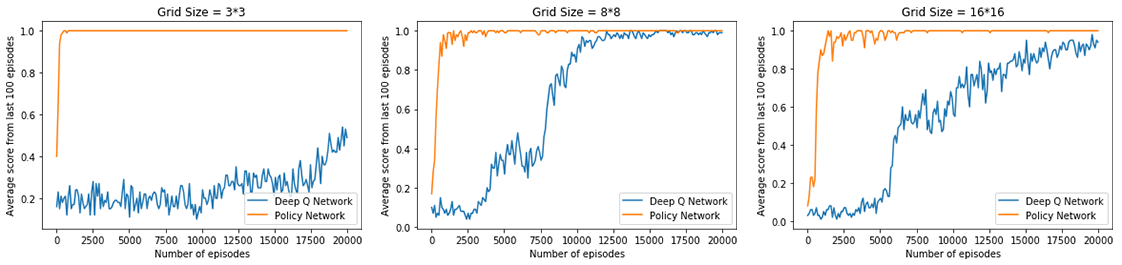
\includegraphics[width=0.9\textwidth]{figures/normal&extream}
    \caption{Normal \& Extreme Task}
    \label{fig:normal_extreme}
  \end{center}
\end{figure}


%------------------------------------------------------------


\section{Discussion}

According to those researchers \cite{DBLP:journals/corr/SchulmanAC17, deepcompareurl}, the result of the experiment indicated that policy gradient has faster convergence rate than DQN, especially in the complexity environment. In the research \cite{deepcompareurl}, it also mentions that policy gradient suffers the high variance in approximately the policy function; it causes the noisy during the estimation. However, we use the variance reduction method to reduce the noise. For this reason, in our experiment result, the policy gradient shows a stable performance from episode to episode.


%------------------------------------------------------------

\section{Conclusions}

In this project, we have deeply understood the history of reinforcement learning. We learn how to implement the two well-known methods, q-learning and policy gradient. Furthermore, we apply those methods in the maze game, and then to training the game agent to reach the goal automatically. During this self-study journey, we also learn the evolutionary process of reinforcement learning, which is a powerful method of machine learning, and it has been utilized not only in the gaming industry but also the robot training. If we have more time, we would like to port our algorithm to different gaming, or even the difficult gaming, such as Pac-man or Mario.

To provide further evaluation of the experiment result of q-learning and policy gradient, the hyper-parameter tuning is extremely important to the accuracy, the average reward and the convergence speed. As same as the other deep learning algorithm, although the method can escape the local optimal, the same value of the parameters can cause the time consumption in each episode.



%------------------------------------------------------------




\bibliographystyle{plain}
\bibliography{cs-seminar}

\section{Roles of the Authors}
We work individually on the reinforcement learning research and algorithm implement, after the research and implement, we share with each other our idea and what we have learned from the reinforcement learning. Therefore, we also help each other to figure out the confusion of the methods and algorithm. in the reporting part, we divide the work as below list.
\begin{itemize}
\item Dongmin Wu: Method, Data, Experiments, Result
\item Shan Kuan: Abstract, introduction, Related work, Discussion, Conclusion, Reference
\end{itemize}
\end{document}
